\section{C) Feature Augmentation}

\subsection{i) Create additional features and train a Logistic Regression model}
This section expands upon Part~A by adding two additional features representing the squares of the original features. This results in the feature vector $\left[x_1,\, x_2,\, x_1^2,\, x_2^2\right]$. This feature engineering can help capture the non-linear nature of the data by transforming the feature space to a higher dimension. A logistic regression model was then trained using these new features.
The feature coefficients are as follows:
\begin{table}[H]
    \centering
    \begin{tabular}{lcc}
        \toprule
        \textbf{Feature} & \textbf{Coefficient} & \textbf{Effect on Prediction} \\
        \midrule
        $x$   & $-0.1500$  & Decreases prediction \\
        $y$   & $6.9671$   & Increases prediction \\
        $x^2$ & $6.4446$   & Increases prediction \\
        $y^2$ & $-0.5419$  & Decreases prediction \\
        \bottomrule
    \end{tabular}
    \caption{Feature coefficients and their effects in the poly LR model.}
    \label{tab:poly_lr_coeffs}
\end{table}


\subsection{ii) Predict target values}
In this higher-dimensional space, the logistic regression model can still find a linear decision boundary, but when projected back to the original 2D scatter plot, this becomes a curved, non-linear boundary. 
This can be seen in Figure 4 below.

\begin{figure}[H]
    \centering
    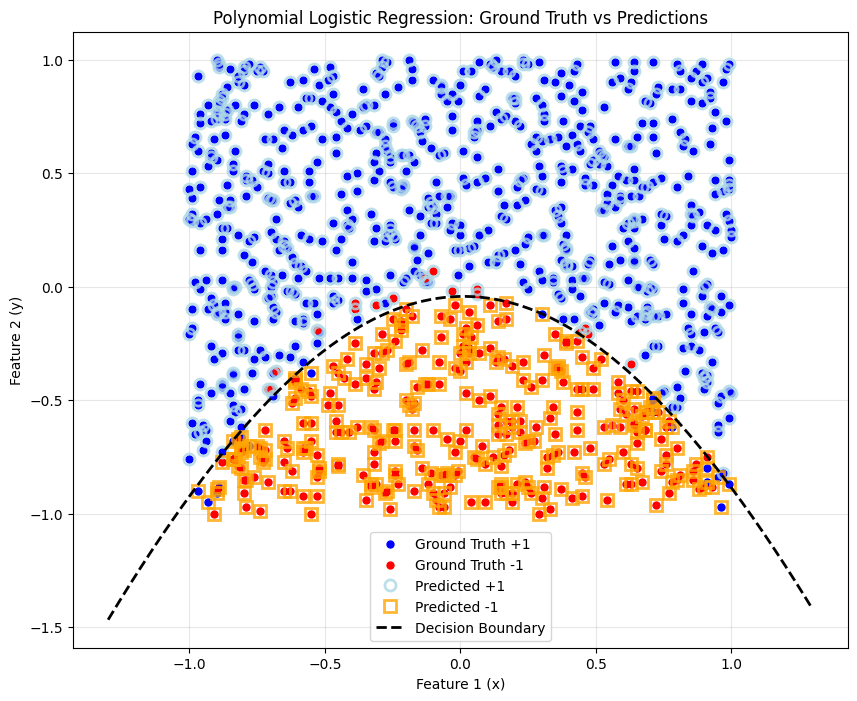
\includegraphics[width=0.8\textwidth]{figures/Poly_LR.png}
    \caption{Logistic Regression Predictions with Polynomial Feature Augmentation}
    \label{fig:Poly_LR}
\end{figure}
\subsection{iii) Compare against baseline}

A simple baseline classifier was created to demonstrate the logistic regression model actually learned something useful. This baseline predictor is a simple majority class classifier, always predicting the most frequent class in the dataset. The polynomial logistic regression model substantially outperforms the baseline, demonstrating that it has learned meaningful discriminatory patterns from the data, as shown in Table~\ref{tab:performance_comparison} below.

\begin{table}[H]
    \centering
    \begin{tabular}{lccc}
        \toprule
        \textbf{Metric} & \textbf{Baseline} & \textbf{Poly LR} & \textbf{Improvement} \\
        \midrule
        Accuracy  & 0.6877 & 0.9640 & +0.2763 \\
        Precision & 0.6877 & 0.9752 & +0.2875 \\
        Recall    & 1.0000 & 0.9723 & -0.0277 \\
        F1        & 0.8149 & 0.9738 & +0.1588 \\
        \bottomrule
    \end{tabular}
    \caption{Performance comparison between baseline and polynomial logistic regression.}
    \label{tab:performance_comparison}
\end{table}


The baseline model achieves an accuracy of $68.77\%$, which reveals that the dataset is imbalanced, with approximately $69\%$ positive samples and $31\%$ negative samples. In contrast, the polynomial logistic regression model achieves an accuracy of $96.40\%$, representing a substantial improvement of $27.63\%$. This significant gain indicates that the model is genuinely learning the underlying patterns in the data, rather than simply exploiting the dataset's class imbalance.

The improvement in precision is particularly noteworthy. The baseline's precision of $68.77\%$ is equal to its accuracy because it always predicts the positive class and never predicts class $-1$, resulting in $31\%$ of its positive predictions being false positives. The polynomial model, however, achieves a precision of $97.52\%$, an increase of $28.75$ percentage points. Recall decreases slightly from $100\%$ to $97.23\%$ (a reduction of $2.77\%$).This shows the model has learned to distinguish between the two classes rather than simply predicting positive for all samples.

The F1-score, which provides a balanced measure of both precision and recall, offers a more comprehensive view of model performance than accuracy alone. The polynomial model achieves an F1-score of $97.38\%$, $15.88\%$ higher than the baseline's $81.49\%$. The baseline's F1-score is artificially inflated by its perfect recall despite poor precision, whereas the polynomial model demonstrates strong performance across both metrics. This highlights how considering a single metric alone can be misleading.

By incorporating polynomial features, the model is able to capture the non-linear decision boundary present in the data. This results in a classifier that meaningfully distinguishes between classes, rather than simply predicting the majority class. The model's ability to maintain high recall ($97.23\%$) while dramatically improving precision ($97.52\%$) demonstrates that it has effectively learned the underlying structure of the data.

\subsection{iv) Bonus}
Unlike the simple linear models where the decision boundary was a straight line, this polynomial logistic regression uses 4 features 
\[x, y, x^2, y^2\].  

The decision boundary occurs where the model's prediction probability equals 0.5. From the coefficient values from Table (4), this gives the following equation: 

\begin{equation}
    0.298 - 0.1500x_1 + 6.9671x_2 + 6.4446x_1^2 - 0.5419x_2^2 = 0
\end{equation}

This equation can rearanged to create a quadratic equation in terms of x2:
\begin{equation}
    -0.5419x_2^2 + 6.9671x_2 + 0.298 - 0.1500x_1 = 0
\end{equation}

This equation can be solved for x2 using the quadratic formula:
\begin{equation}
    x_2 = \frac{-6.9671 \pm \sqrt{6.9671^2 - 4 \cdot -0.5419 \cdot (0.298 - 0.1500x_1)}}{2 \cdot -0.5419}
\end{equation}

giving two solutions, only one of which is valid and plotted in Figure 4.